\chapter{INITIAL PLANNING \& INFORMATION GATHERING}\label{chapter:initial_planning_and_information_gathering}
This chapter will explain how the initial planning was done by describing activities at the project's beginning. After that, the information-gathering activities of the project will be explained. In addition, the most important finding from the information-gathering activities will be presented.

\section{Initial planning}
This section will explain how the initial planning of the project was done. In the beginning, the front end of the project will be explained. After that creation of the meta-plan will be laid out. Finally, it is described how the rest of the work was finally being made.

\subsection{Beginning of the project}\label{subsection:beginning_of_the_project}
The M-Files \gls{qa} team originally initiated the test automation project. In the beginning, it was thought that the project would mainly consist of the construction of the integration and system-level test automation systems. Based on the assumptions, even some very rudimentary plans were made regarding those test levels.

However, those impressions did not last long. Shortly after the project's initiation, a meeting with a Hubshare development team was kept. After the meeting, it was evident that Hubshare's needs were significantly broader compared to initial beliefs inside \gls{qa} team. During the meeting, many wishes were presented regarding test automation, further refined in the meta plan explained in the following subsection.

\subsection{Creation of the meta-plan}
Because the project size ended up being extensive, it was impossible to start planning immediately. Instead plan on how to plan, the so-called "meta-plan" was first needed. In the meta-plan, the scope of the thesis was initially roughly presented using a list of things that will and will not be addressed as well as things that may be addressed during the thesis. Another vital aspect described in the meta-plan was the plan for the information gathering. In addition, the meta plan included some rough proposals of the project's phases and thesis' structure. Finally, the meta-plan also included a list of technical tools that will be used during the project.

\subsection{Ways of working}\label{subsection:ways_of_working}
At the beginning of the project, tasks were mainly done using the waterfall-like process method (processes described in the \autoref{subsection:test_automation_daily_activities}). This process model was implicitly chosen because it took time to understand the exact tasks at the beginning of the project. In the agile-based methods, it would have been hard to fill the backlog appropriately. As a result of the waterfall-like process, the most vital details of the test automation system, like processes and architecture, were initially planned.

However, as described in the \autoref{subsection:test_automation_daily_activities}, the waterfall model has the inherent flaw of not being flexible, and due to that, it is important not to over-plan. Because of this, only high-level architectures of the test automation systems were planned, and implementation-specific details were left open. In addition, it was always kept in mind that things can and will change, and none of the plans should be considered final.

After the initial phase, the way of working was changed radically towards a more agile way, where things were developed in smaller cycles with faster iterations. More dynamic iterations were now possible because, during the initial planning, general directions in the test automation project were established. So overall, the project followed a hybrid approach between the waterfall and agile models.

\section{Literature reviews}\label{chapter:literature_reviews}
As described in the \autoref{subsection:literature_review}, an academic literature review was used during this thesis. However, additionally, multiple other literature sources were used during this research. The usage of different literature sources is defined in the following sub-sections.

\subsection{Prior M-Files theses}
M-Files is a famous company for thesis workers. Overall about 20 theses have been done for M-Files during the years. Many of the theses have been testing and test automation related. Due to that, other theses were also helpful as a reference for this project. Because by academic conventions, theses are not appropriate sources for academic research due to more tremendous changes of mistakes contained within them. Due to that, other M-Files theses were not directly affiliated with this research and were only used as references to guide this thesis towards the correct direction.

\subsection{M-Files process \& test automation documents}
M-Files has an extensive collection of process documents that describe how current M-Files processes work. Process documents were helpful as a reference for constructing new test automation processes for Hubshare. In addition, some documents did describe M-Files' existing test automation systems. Those documents were helpful during the creation of the Hubshare test automation architecture.

\subsection{Grey literature reviews}
Even though existing M-Files test automation systems and documentation provided an excellent basis for a new test automation system, those systems were initially designed several years ago. In the meantime, test automation processes and technologies have been advancing. To take advantage of the newest technologies relying on already done work was insufficient.

White paper literature does provide knowledge about the test automation processes and ways of selecting the perfect test automation tool for the purpose. However, the white paper literature does not provide direct information about the current state-of-the-art test automation tools. Instead, this information is readily available in the grey page literature. Because of that, the grey page literature review was used to identify the current best test automation tools available for a particular problem. Grey literature research has also been used by other researchers for similar purposes \cite{paivi2017choosing,ricca2021web}.

\section{Code reviews}
During information gathering, two types of code reviews were made. The first code review concentrated on the M-Files' existing test automation, while the latter code review concentrated on Hubshare's code base. More information about the code reviews is available in the following sections.

\subsection{M-Files test automation code reviews}
While M-Files' existing process and test automation documents already provided plenty of information about the state of the M-Files test automation, every tiny detail was not still included in the documentation. To fully understand test automation, it was necessary to read and play with the code available in the existing test automation systems. Even though with an extensive review, it would have been possible to extract a significant amount of technical information from the code base, the code review was done only on a superficial level due to the higher level scope of this thesis. So the code review mainly concentrated only on the architectural aspects of the system.

\subsection{Hubshare code base reviews}
In addition to understanding a realistic test automation system, it was necessary to understand how Hubshare's product worked internally. Without knowledge of Hubshare's code base, it would have been hard to design a sound test automation system. Additionally, designing especially lower-level test automation systems like unit testing would have been impossible. A proper lower-level understanding was necessary because unit test automation is close to the implementation details and can only be adequately constructed by understanding the code. So deep enough code review was carried out so that the application's architecture could be understood and some of the possible test automation problems could be predicted.

\section{Interviews}
Interviews were one of the primary information-gathering methods during this thesis. Overall, eleven interview sessions were kept during the creation of this thesis. In the following sub-sections, interviews will be explained in detail.

\subsection{Planning of the interviews}
All interviews were planned based on the information needs identified during the other information-gathering activities. Questions of the interviews were tailored to the specific professional being interviewed so that the interviewee could provide a comprehensive answer to the questions. Because the interviews were primarily used for general information-gathering purposes, there would not have been any advantage of having the same interview questions for everyone.

Interview questions were made fairly open-ended in a true semi-structured interview fashion. As an example, one of the questions asked from the Hubshare developers was: "How do you feel about test automation?". Interviewees can answer broadly to these open-ended questions, which is good because answers can lead to surprising results, based on which the discussion can be directed in new and exciting directions. The selected interview questions can be found in the \autoref{appendix:interview_questions}. The appendix includes all the vital review questions from the thesis point of view while omitting specific technical questions from certain parties that are not important for this work.

\subsection{Selection of the interviewees}
The selection of the interviewees was made based on the thesis research questions. Different interviewees from various backgrounds were selected to cover the thesis subjects as broadly as possible. The final interviewees were the best available experts from their fields.

\subsection{Interview sessions}
Interview sessions were between 30 and 90 minutes, depending on the information needed from a particular professional. Interview sessions started with the introduction of the interviewer and the project. After the introduction, the interview began with a set of questions. Questions were mainly asked in order, but in between the questions, some ad hoc follow-up questions could be asked if the interviewer noticed some interesting new subjects while the interviewee was answering the previous question. Finally, as described in the \autoref{appendix:interview_questions}, it was also asked whether the interviewee had anything to add that could be helpful for the project. Finally, the interviewee was thanked for her/his help, and the interview ended.

During the interview, notes from interesting answers were taken. Interviews were not recorded nor transliterated. The recording was not used because that could have negatively affected the interview by making the interviewee unnecessarily uncomfortable. Recording the interviews would have probably slightly increased the data input gathered from the interviews by making sure that no details could have slipped by. However, it was not seen as especially important during these interviews because the idea was to chart different fields of the subject, not investigate precisely one interviewee's opinions and thoughts.

\subsection{Management key findings}\label{subsection:management_key_findings}
According to Hubshare's main \gls{qa}, the lack of proper regression test automation is currently the most critical testing-related aspect that should be improved. Based on Hubshare's \gls{po}, appropriate time must be reserved to realise new test automation cases in the future. \gls{po} also emphasised the importance of different stakeholders when considering automation of the test cases.

In addition to Hubshare-related personnel, M-Files' agile coach gave many valuable management-related suggestions. Based on the interview, during management design, it is essential to consider who "owns" test cases so that the test cases can be efficiently supported and improved in the future. Also, according to him, unit tests should be part of the daily development process and considered while implementing a user story.

The agile coach also emphasised appropriate test automation education. According to him, it is often a cultural challenge that developers focus entirely on the developing, while \gls{qa}'s focus entirely on the testing. Coach stated that in the ideal world, it would be good if the developer would implement test automation cases during the user story development with \glspl{qa} assisting or coaching the developer. M-Files system testing expert also shared this view. Education should be arranged for both developers and testers to achieve the desired state. However coach mentioned that, even with sufficient education, change takes time because both the behaviour and mindset of the developers and \gls{qa} engineers must be altered before the adoption is fully complete. Because the change requires time, it is not feasible to start with too grand changes, and great methods like \glsfirst{tdd} introduced in the \autoref{subsection:test_automation_daily_activities} are out of the question for the beginning.

Additionally, the agile coach mentioned some methods to catch the test automation-related technical loan. The first way is to organise focus sprints, but the organisation may be hard to fit into the calendar. The second possibility is to improve test automation near regressions. This approach requires a smaller initial time investment but is slower.

A system test automation expert mentioned that customer viewpoint should be considered while developing new test automation cases, especially in scenarios important for customers. Especially system-level test cases should be done from the customer's viewpoint.

\subsection{Technical key findings}
Based on the interview with the M-Files unit testing expert, it is wise to have hand-crafted separate easy-to-use mocks for commonly used functionality. This way, developers can quickly mock the functionality they want while developing new test cases. The unit testing expert also said that it should be easy for the developers to track the application's state during unit testing to aid the assertion of the results.

The unit testing expert also gave tips on what to avoid while designing a new unit testing framework. Unit tests should be independent, and the execution order should be indifferent. Names of the test cases should clearly describe the thing that the test is trying to verify. The test case setup should not be entangled with the test case and should instead be clearly visible.

During an interview with the integration testing expert, it was mentioned that automatic environment generation had been a helpful feature in the integration testing framework, which makes it possible to run the same tests in different environments. Another helpful feature in the integration testing framework is isolation between test cases, which prevents side effects. According to a unit testing expert, it would also be good if the integration testing framework had a more straightforward developer setup.

Based on the M-Files system testing expert's review, it is good that frontend-based system test automation cases are fast, so that regression bugs are found swiftly. However, based on the expert, it is still a good idea to consider using frontend unit tests for some scenarios to save on operational expenses of the test automation.

From the \glsfirst{ci} point of view, M-Files \gls{ci} specialists stated that stable and reproducible \gls{ci} is the most important thing. \gls{ci} should also have sufficient logging so that failures in the \gls{ci} can quickly be investigated after test runs have been completed. \gls{ci} pipelines should be easily executable by the developers so that new user stories can be easily tested using the \gls{ci} pipeline.

\section{Survey}
This section will explain how the "State of the M-Files test automation survey" was created and executed and what the survey's key results were. The first two subsections will concentrate on the planning and execution of the survey, while the latter three will present the survey results.

\subsection{Planning of the survey}
Initially, the survey was strictly created from this thesis point of view and included only some strictly technical questions. In the original version, only technical questions were included because it was thought that enough information from management-related matters was already collected using other methods. Also, it was thought that the target demographic, developers, would be most eager to answer the technical questions.

However, sometime after the initial draft of the survey was made, it was realised that the results of this survey could also be valuable for the other M-Files' test automation efforts. Because of that, a small task force consisting of test automation experts was formed. A task force was selected as an approach because there was a need to collect ideas efficiently from a small group of people. Using the task force rest of the survey questions were planned during a workshop session in which the creation of the new questions was elicitated using silent and loud brainstorming techniques.

The final form of the questions was constructed using survey planning best practices, including minimal question length and balanced answering alternatives. Most of the multiple choice questions used a six-grade Likert scale. The Likert scale is a way to measure human attitude towards certain subjects using an ordered set of statements \cite{joshi2015likert}. Six-point Likert scale was chosen because it forced respondents to select an opinion instead of staying neutral and provided enough options to express the opinion effortlessly. The best number of Likert points has also been debated in the literature, but no definitive conclusion has been made so far \cite{edwards2014effects,garland1991mid}. The final survey did contain 35 questions overall.

\subsection{Execution of the survey}\label{subsection:execution_of_the_survey}
The link to complete the survey was sent to the whole M-Files product development staff. Initially, the link was sent via email and internal chat groups. These information channels were selected because they are the primary communication channels used by the employees. While the survey was open multiple reminders about the survey were sent so that a sufficient amount of answers could be collected. Overall the survey was open for 11 days.

Almost all of the survey questions were optional because not all respondents could answer all of the questions. All questions were not answerable due to the highly varying roles of the respondents. There were only three general questions that were obligatory. Exact information about the mandatory and optional questions can be found in the \autoref{appendix:survey_questions}.

\subsection{Survey key metrics}
Overall the survey received 60 answers. As seen from the \autoref{fig:survey_key_demographics}, most respondents were developers and had been working for M-Files for five years or more. The average response time was 18 minutes.

\begin{figure}
	\centering
	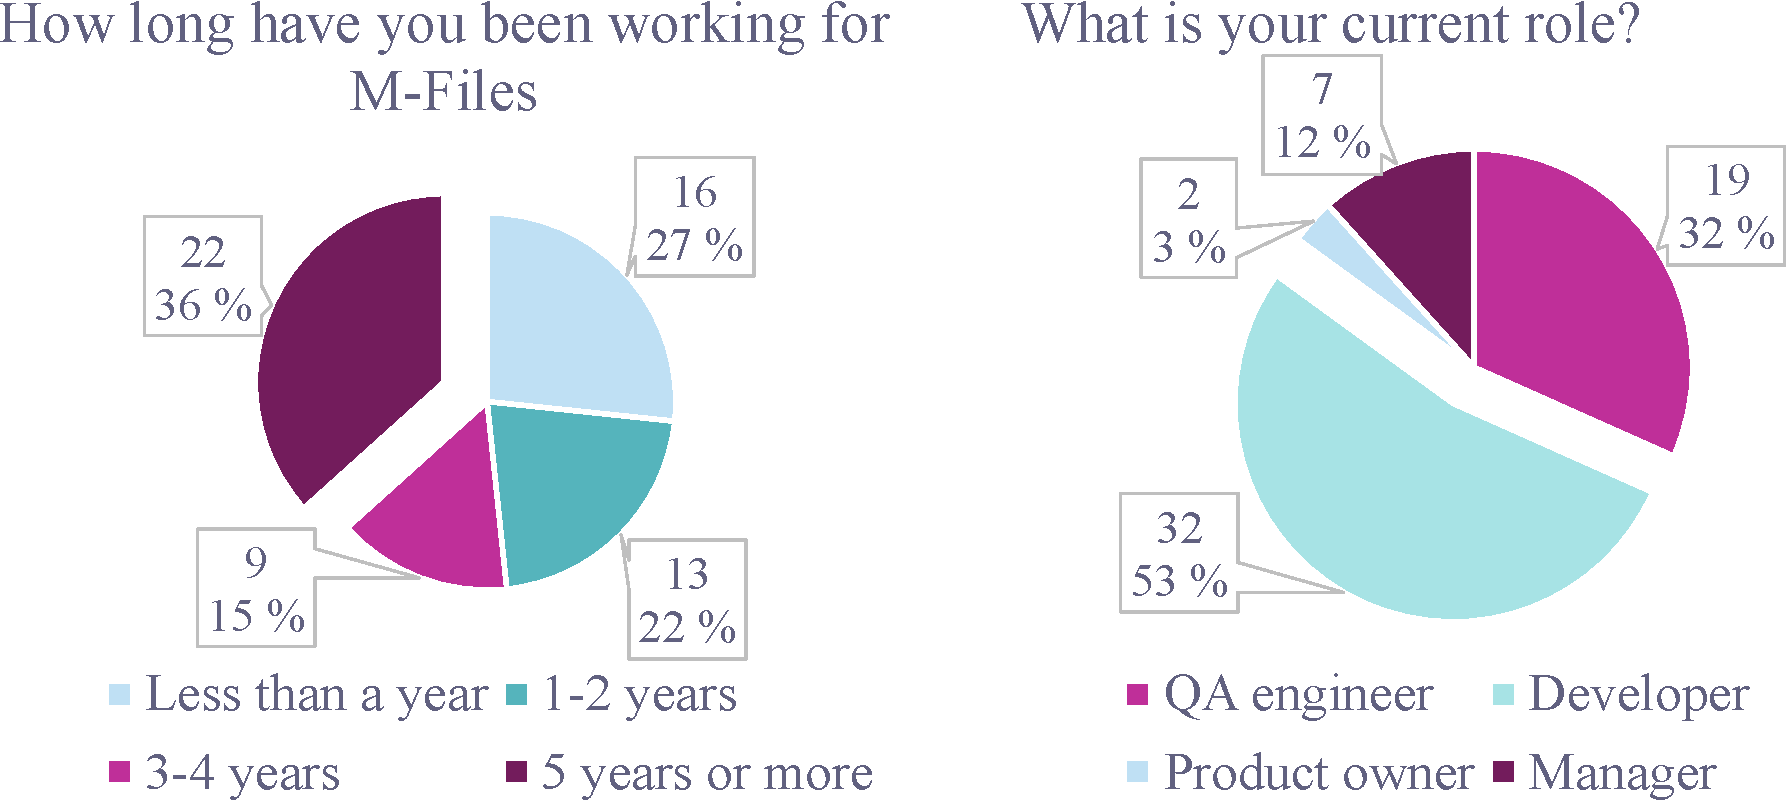
\includegraphics{Survey_key_demographics}
	\caption{Survey key demographics}
	\label{fig:survey_key_demographics}
\end{figure}

Survey's answer rate was 26\%. Due to a fairly low answer rate, this survey can provide only indicative results from the actual situation. However, from the context of this research, a low answer rate is not critical because this thesis aims to capture only significant directions instead of specialising in the last-minute details.

As stated in the \autoref{subsection:execution_of_the_survey}, most survey questions were optional. Regardless of optionality, most of the multiple-choice questions were answered by all respondents, as seen from the \autoref{fig:per_multiple_choice_question_answer_rate_bar_chart}. Only some open questions related to multiple choice questions at the end were not that actively answered, which was expected given that answer to a related open question was also required.

\begin{figure}
	\centering
	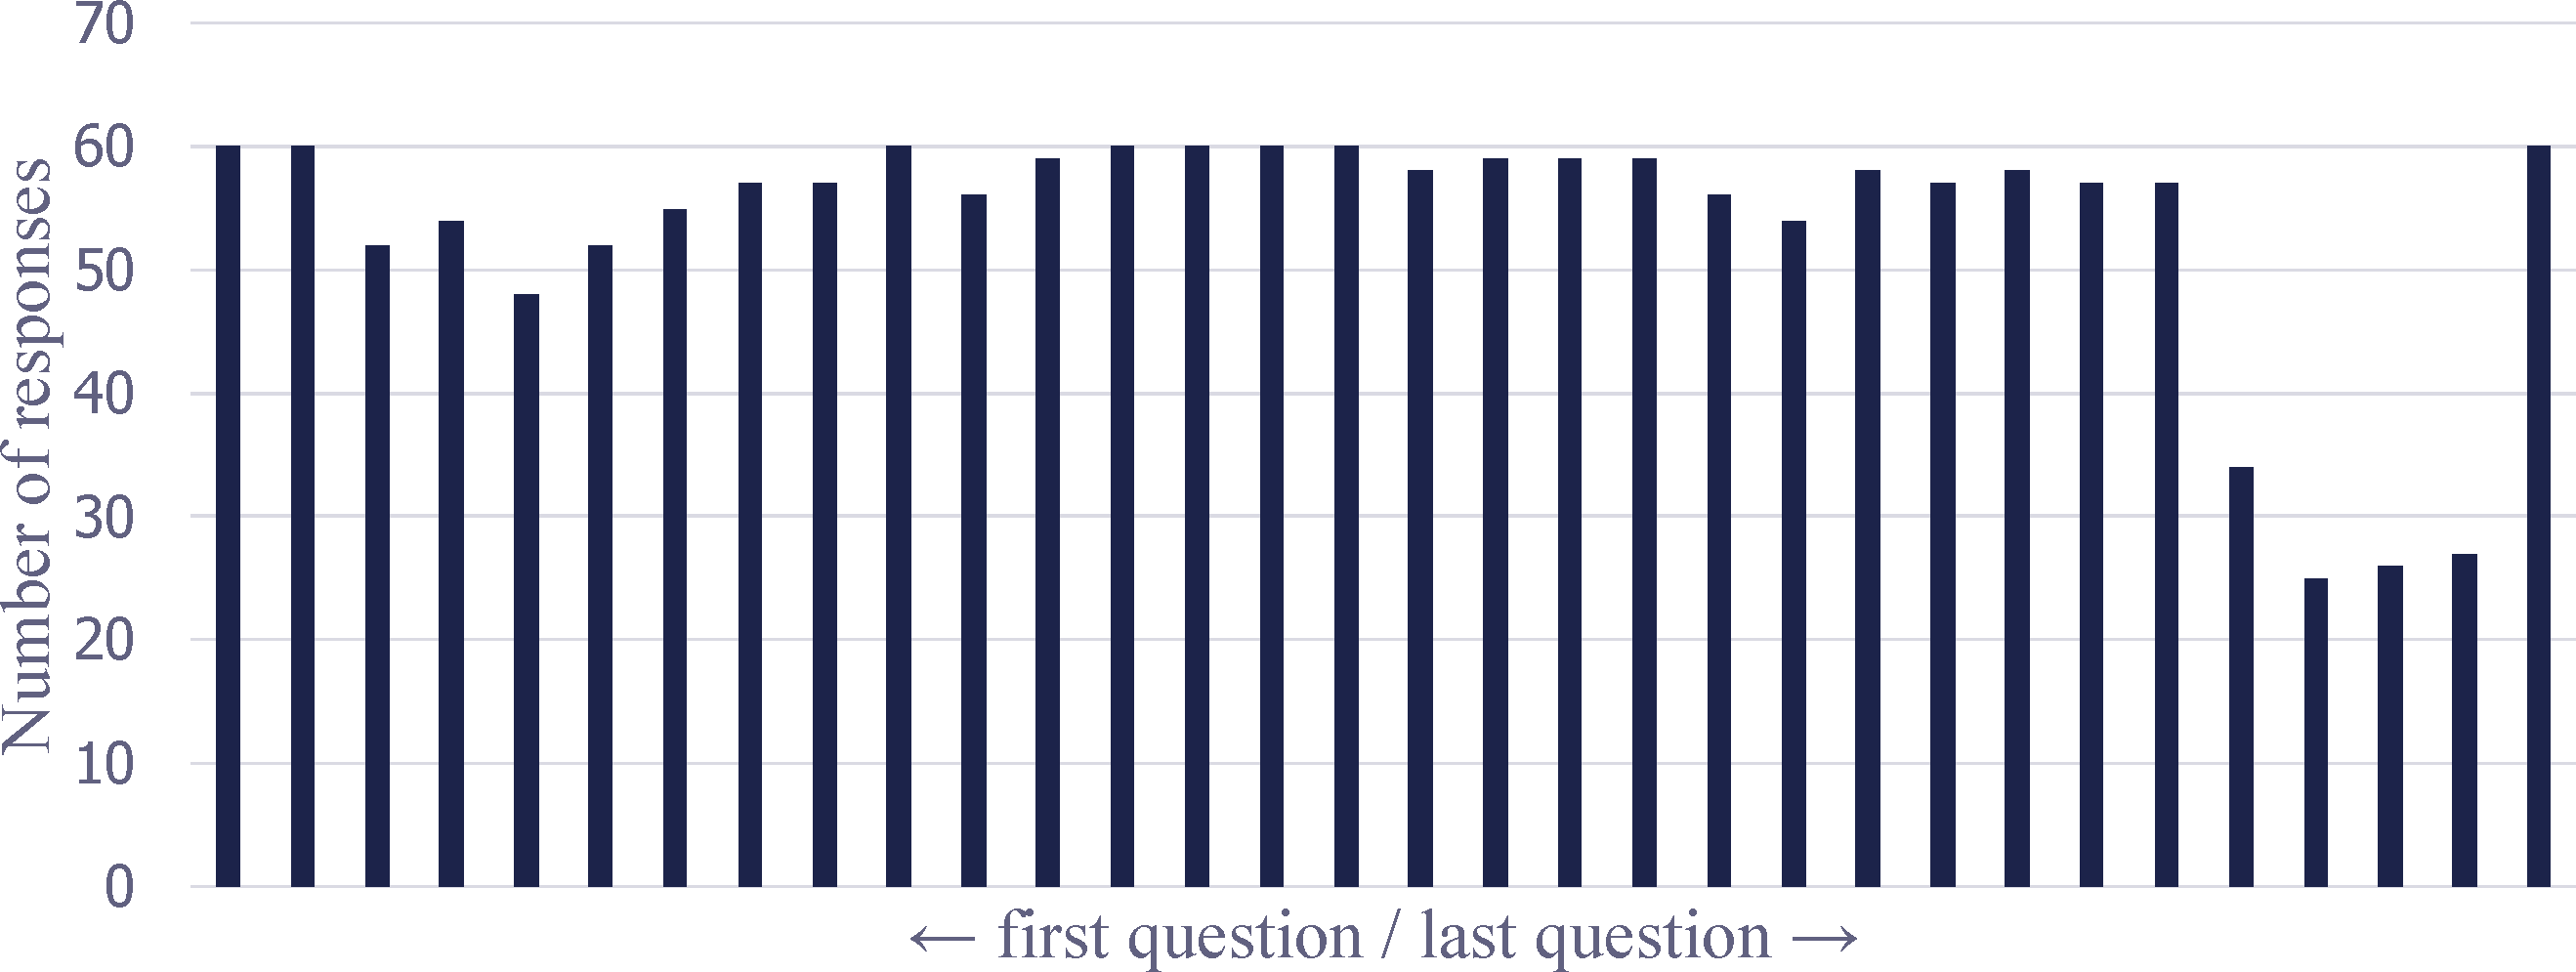
\includegraphics{Per_multiple_choice_question_answer_rate_bar_chart}
	\caption{Per multiple choice question answer rate bar chart}
	\label{fig:per_multiple_choice_question_answer_rate_bar_chart}
\end{figure}

With the open questions, the answering situation was different. As seen from the \autoref{fig:per_open_question_answer_rate_bar_chart}, the first open question collected roughly 40 responses, while the last question was answered only by ten respondents. Answer rates were not surprising because the survey was long, and respondents' concentration decreased towards the end of the survey. The decrease in answer rate has also been identified in the literature previously \cite{burchell1992effect}. The effect was also visible in the responses themselves. Answers to the first questions were longer and contained clauses even for the other questions, while later answers were shorter and provided only to-the-point details. In addition, response rates are affected because later questions were more challenging and more technical, making questions tricky or even impossible to answer for some respondents.

\begin{figure}
	\centering
	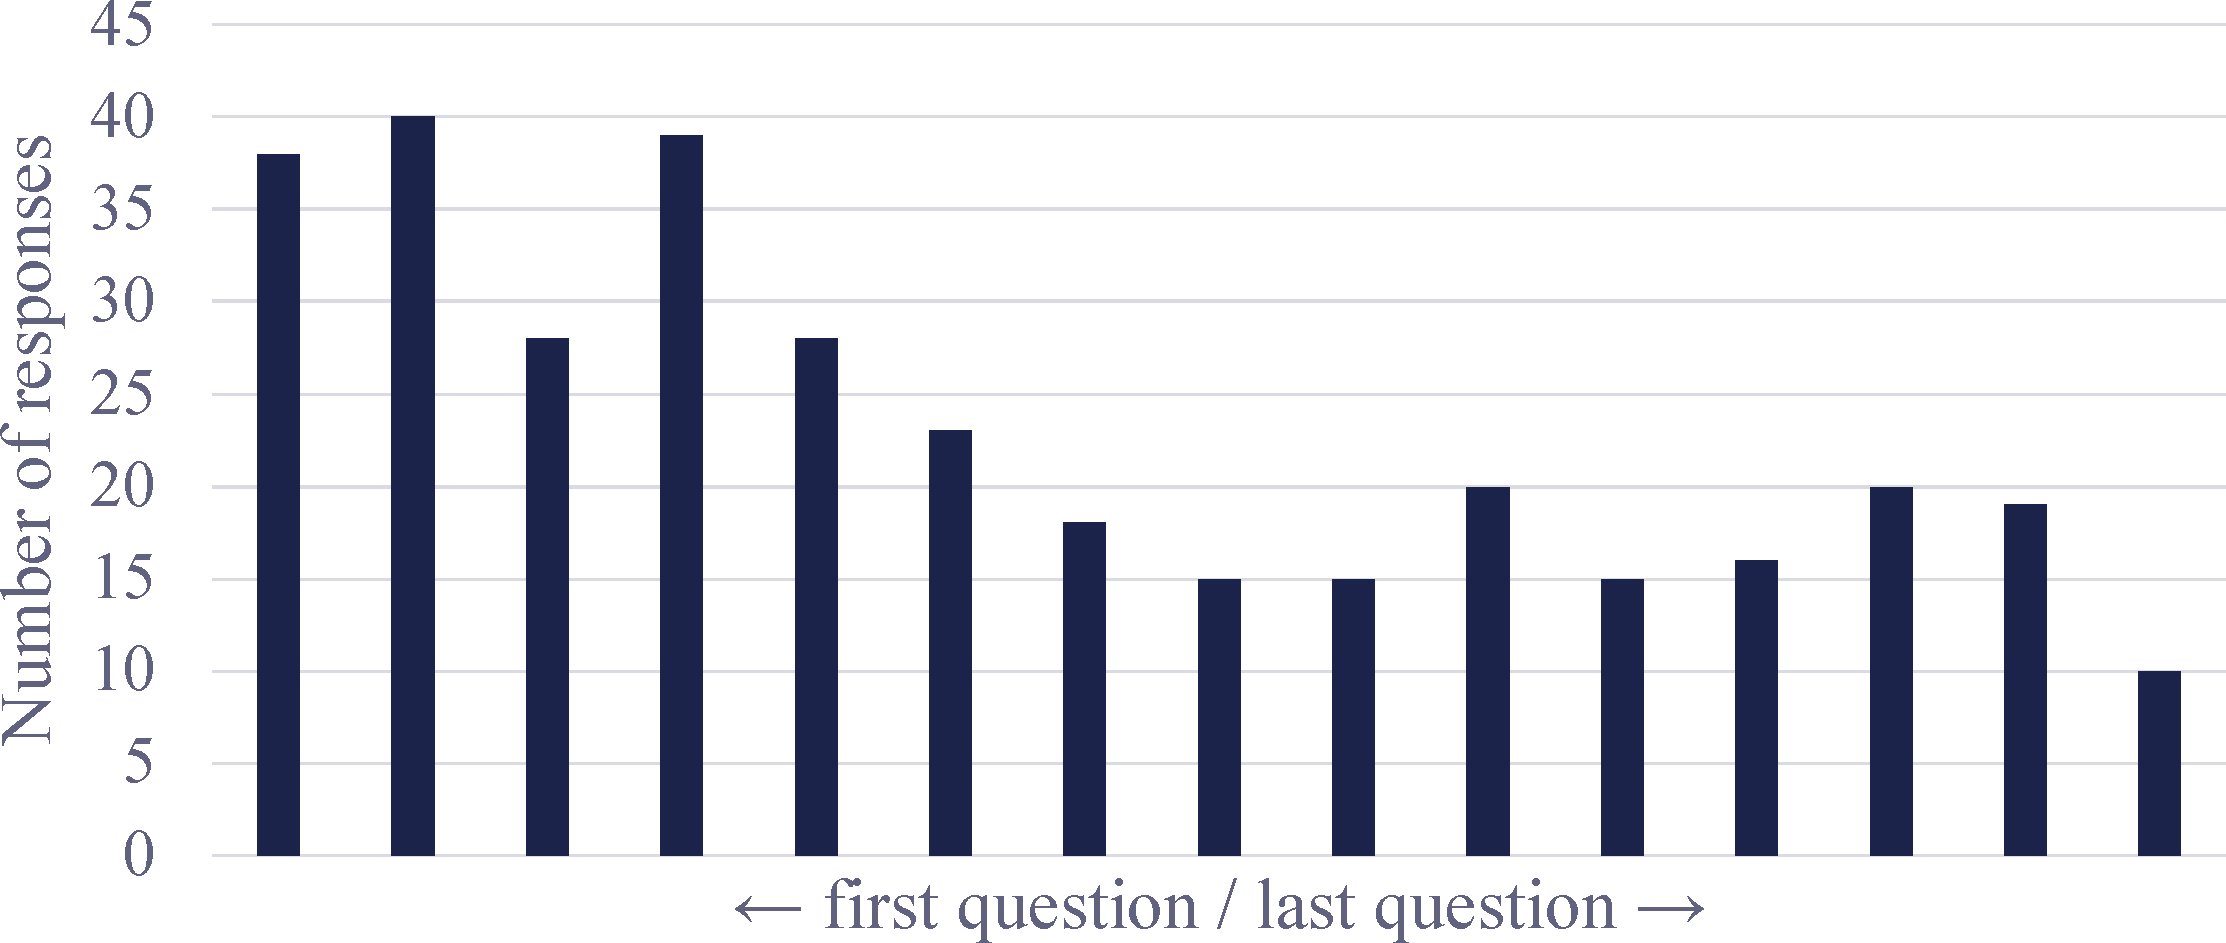
\includegraphics{Per_open_question_answer_rate_bar_chart}
	\caption{Per open question answer rate bar chart}
	\label{fig:per_open_question_answer_rate_bar_chart}
\end{figure}

\subsection{Management key findings}
\autoref{survey_question:works_well_in_processes} about the current test automation processes' positive aspects was directly related to the management. Unfortunately, something was wrong with the formulation of the question, and respondents provided all kinds of answers to the question. Many wrong answers were probably provided for the question because the question was first in the survey, and its formulation was too open-ended. Fortunately, also, some proper responses were given. Based on the answers, especially agile processes, normal execution of the test automation cases was liked in the current process. In the follow-up \autoref{survey_question:does_not_work_well_in_processes} that asked about negative aspects, some respondents answered that the development teams should be more in charge of the test automation improvements and that the new test automation case development could be started earlier in the user story.

Answers related to \glsfirst{dod} improvements (\autoref{survey_question:how_dod_can_be_improved}) were interesting. While writing this thesis, M-Files did have quite simple \gls{dod} that plainly stated that the test automation cases should have been implemented. Because of that, it was expected that there would be only improvement suggestions. However, many respondents preferred current simple \gls{dod}, which was unexpected. However, also improvement ideas were given. For example, it was suggested that there could be \gls{dod} point for the test coverage and a point for explaining why some test automation cases were not done.

\subsection{Feelings \& attitudes key findings}\label{subsection:feelings_and_attitudes_key_findings}
Test automation confidence-related questions did have fairly classical answers (\autoref{survey_question:test_automation_confidence}). Respondents stated that good coverage, reliability, test automation framework clarity and automation's ability to catch errors not visible locally were important aspects providing confidence to test automation. On the other hand, low coverage, flakiness of the test cases and poor test case quality decreased confidence in test automation.

For the test automation value question, \autoref{survey_question:test_automation_value}, respondents stated that especially reduction of the manual effort and testing of the hard-to-test cases provided value for them. On the other hand, things like unreliable and case execution speed decreased test automation value for them.

The reasons for attitudes towards test automation were charted in the \autoref{survey_question:test_automation_attitude}. As increasing factors, at least the following things were mentioned: reduced manual effort, enabling \glsfirst{cd}, reduction of regression bugs, and enabling velocity without burn-out. As decreasing factors, the following aspects were mentioned: lack of training, the complexity of mocking, hard-to-pinpoint failure location and reliability of the environment.

\subsection{Education key findings}
One of the more surprising results of the survey was visible in the \autoref{survey_question:sufficient_test_automation_knowledge} that asked whether the respondent believed that she or he has sufficient knowledge to do test automation cases. Higher than expected number of respondents answered no to the question. The percentage of no answers was surprising because test automation is generally heavily used at M-Files, and the number of yes answers was expected to be very high. The results emphasise the importance of explicit training related to testing automation.

Based on the \autoref{survey_question:preferred_ways_of_learning} results seen in the \autoref{fig:which_way_would_you_like_to_learn_more_about_the_test_automation_bar_chart} preferred way of learning more about the test automation are training sessions. Also, workshops and better documentation related to testing automation are good education alternatives. Test automation champions and tutoring were less exciting learning possibilities for the respondents.

\begin{figure}
	\centering
	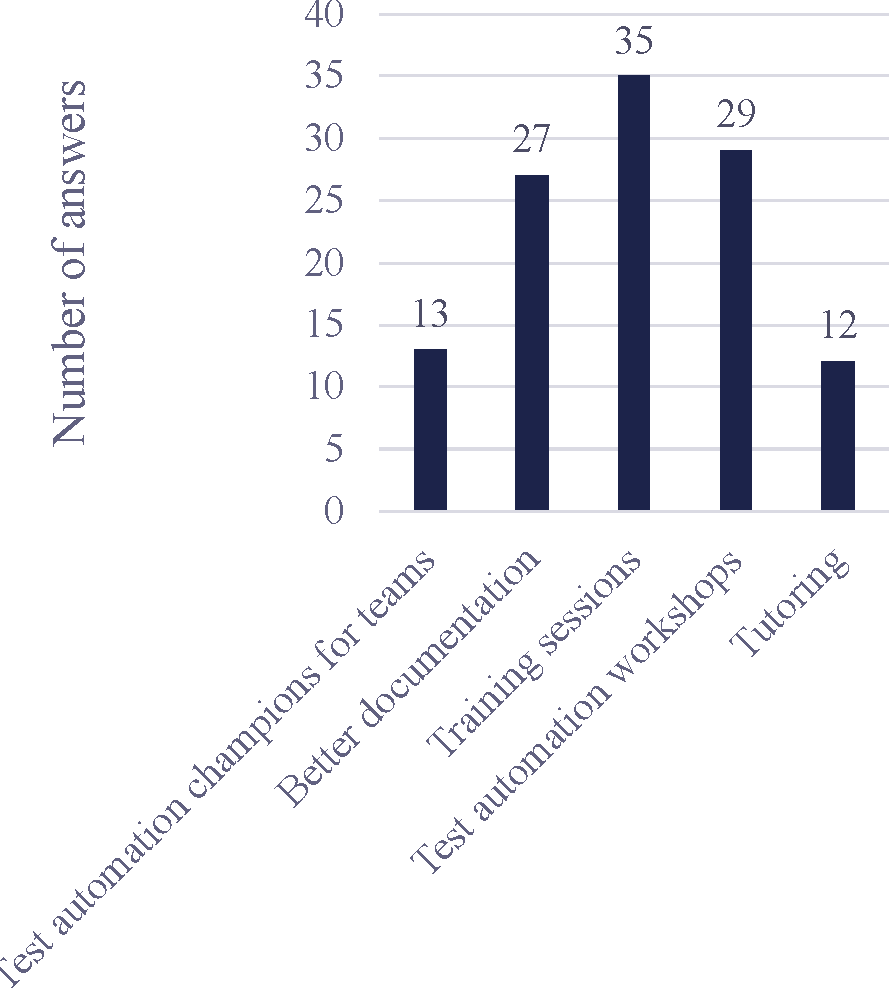
\includegraphics[width=0.6\textwidth]{Ways_of_learning_bar_chart}
	\caption{Answer's distribution for the question: Which way would you like to learn more about the test automation?}
	\label{fig:which_way_would_you_like_to_learn_more_about_the_test_automation_bar_chart}
\end{figure}
\FloatBarrier

\subsection{Technical key findings}\label{subsection:technical_key_findings}
In the \autoref{survey_question:importance_of_test_automation_ascpects}, it was asked how important certain aspects are in test automation. As seen from the \autoref{fig:how_important_following_test_automation_aspects_are_for_you_bar_chart}, all asked aspects were crucial for the respondents. However, especially reliability of the automation and clear error messages were vital for the respondents, which was also visible in the \autoref{subsection:feelings_and_attitudes_key_findings}. Ease of development, environment setup and execution speed were slightly less critical aspects based on the responses.

\begin{figure}
	\centering
	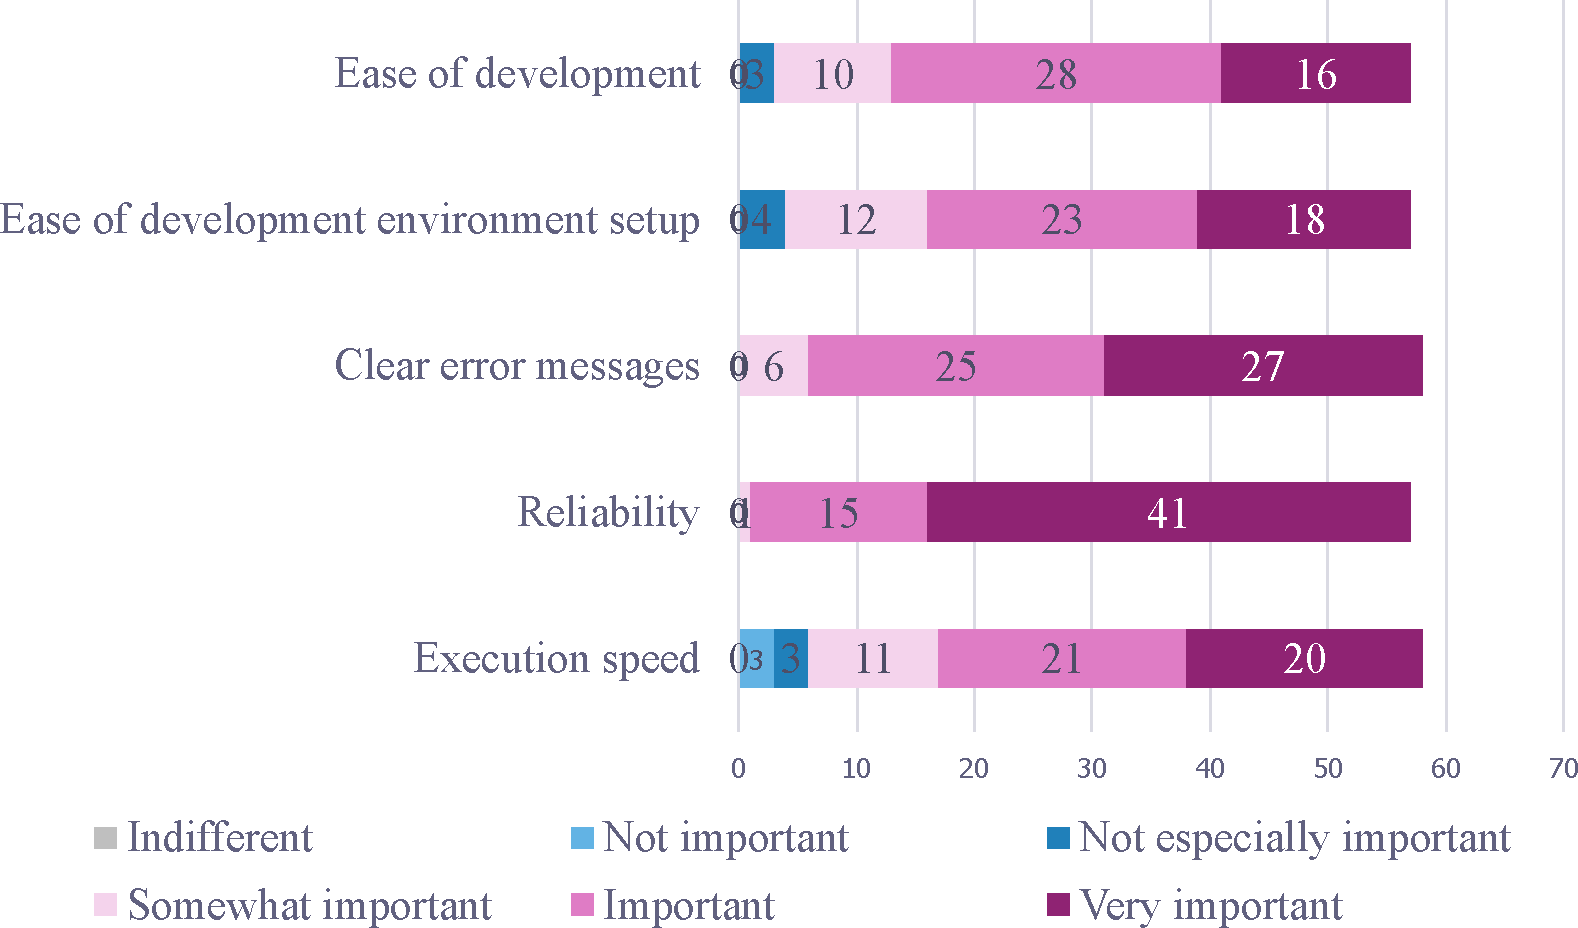
\includegraphics{Importance_of_test_automation_aspects_bar_chart}
	\caption{Answer's distribution for the question: How important following test automation aspects are for you?}
	\label{fig:how_important_following_test_automation_aspects_are_for_you_bar_chart}
\end{figure}

Respondents especially liked the fast running time and good logging of unit tests, based on the responses to unit testing-related questions (\autoref{survey_question:good_in_unit_test_automation}) and follow-up questions. Some respondents described unit tests as easy to set up, run, write and debug. Unit tests were also described to be reliable. However, some respondents also said that the tests were hard to write and required initialisation code to write them was too complex. In addition complexity of mocking, hard-to-understand test steps and clarity of the test results hindered unit testing.

Responses to \autoref{survey_question:good_in_integration_test_automation} and follow-up questions related to integration test automation mentioned that reliability of the local test runs and integration to cloud services was seen as an advantage of existing integration testing. However, flakiness, slowness, long queue times, hard-to-read logs and gaps in the documentation has been seen as a hindrance to the integration test automation development.

Generally, \gls{ui} test automation was liked based on the results for the \autoref{survey_question:good_in_ui_test_automation}. Especially structure, reliability and speed of the test automation were liked. However, some respondents still stated that test execution speed could still be improved and the flakiness of the test cases reduced.

Respondents liked the triggering and labelling system as well as the high configurability of the pipeline, based on the responses to \autoref{survey_question:good_in_pipelines} and follow-up questions related to \gls{ci}. However, most of the respondents stated that pipelines generally run too slowly. In addition, it was mentioned that documentation related to pipeline parameters could still be improved, and some would have also liked to see more parameters for enabling additional logging.